\documentclass[a4paper,11pt]{article}

% Identificação
\newcommand{\pbtitulo}{Estatística}
\newcommand{\pbversao}{1.1}

\usepackage{../sty/tutorial}

%----------------------------------------------------------------------
% Início do Documento
%----------------------------------------------------------------------
\begin{document}

\maketitle % mostrar o título
\thispagestyle{fancy} % habilitar o cabeçalho/rodapé das páginas

%----------------------------------------------------------------------
% RESUMO DO ARTIGO
%----------------------------------------------------------------------

\begin{abstract}	
\initial{N}a metade do século XIX, a humanidade estava em estado de apoteose com as descobertas científicas, uma grande onda de otimismo tomou a Europa com as novas possibilidades. Parecia uma questão de tempo até que aprendêssemos todas as leis que regem a natureza. Tivemos grandes progressos na Física, na Biologia e Astronomia que justificavam esse excesso de otimismo. Parecia que se tivéssemos boas medições poderíamos descrever e prever qualquer coisa. Bom, não preciso dizer que os positivistas estavam errados, mas vamos fingir que não sabemos e continuar nossa história. \textbf{Estatística} é o estudo ou um conjunto de técnicas que permite de forma sistemática coletar, organizar, descrever, analisar e interpretar observações advindas de diversas origens afim de extrair conclusões. Estatística é ambos, parte ciência da incerteza e tecnologia da extração de informações. Nos auxilia a tomar importantes decisões.
\end{abstract}

%----------------------------------------------------------------------
% CONTEÚDO DO ARTIGO
%----------------------------------------------------------------------
\section{História}
No século XVIII, ao fazer algumas medições da posição dos planetas, os cientistas notaram alguns pequenos desvios. Esperava-se que o planeta estivesse em uma determinada posição e estava no \textit{lugar errado}. Havia duas possíveis explicações para esse fenômeno: o modelo estaria errado ou os equipamentos que coletavam as observações não eram precisos o suficiente. O modelo parecia conciso então a culpa devia ser dos instrumentos e assim começaram a produzir equipamentos cada vez mais refinados. Ao analisar esses desvios, foi observado que seguiam sempre uma certa distribuição. \textit{Laplace} dedicou um volume inteiro das suas predições astronômicas apenas para tratar sobre esses erros, conhecemos esses trabalho na atualidade por \textbf{Distribuição Normal}.

A partir da melhora na precisão dos equipamentos e conforme esperado, os erros diminuíram, e isso incentivou a criação de equipamentos cada vez melhores. Porém conforme se tornavam cada vez mais precisos, começou a acontecer um fenômeno estranho: \textbf{os erros, ao invés de diminuírem, passaram a aumentar!}. Os cientistas se perguntaram qual seria a causa disso? Nosso mundo não é \textbf{determinístico}, mas sim \textbf{estocástico}, ou seja, os eventos possuem uma característica aleatória. Mesmo que existam os mais precisos equipamentos e conhecêssemos o modelo mais perfeito da natureza, ainda assim não seria uma garantia de boa predição, ocorrem fatores aleatórios que não controlamos.

\textit{Francis Galton} foi um gênio em diversas áreas, e antes de mais nada um excepcional observador. Foi um dos primeiros a notar outra importante característica sobre as distribuições que é a forma da sua dispersão, ou seja, enquanto a média passa ideia de centralidade, a dispersão nos diz o quanto as observações estão distribuídas longe da média, daí a ideia de \textbf{Variância} e \textbf{Desvio Padrão}.

Galton fundou um laboratório para coletar e tabelar diversas características humanas, foram 6 anos de análise e 9.000 famílias. A mesma distribuição de erros observadas nas medições astronômicas foi encontrada outras vezes como na altura das pessoas ou no tamanho dos antebraços. Ao perceber que quando a altura média dos pais era muita alta (ou baixa), seus filhos deveriam ser também mais altos (ou baixos) que a média.
\begin{figure}[H]
	\centering
	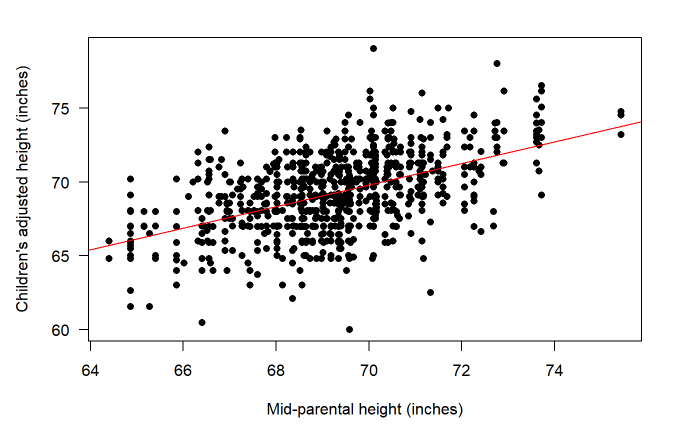
\includegraphics[width=0.8\textwidth]{imagens/galtonDataset.png}
	\caption{Estudo de Galton}
\end{figure}

Percebeu que existia um comportamento escondido e que esses filhos dificilmente chegavam a ser tão altos (ou baixos) quanto seus pais, parecia existir uma força puxando a altura dos filhos de volta a média. Essa força foi chamada de \textbf{Regressão}.

\subsection{Minha história com Estatística}
Sou formado formalmente através de uma Pós-Graduação de Estatística Avançada, porém creio que o que mais me atraiu foi o livro \textbf{Como Mentir com Estatística} (1954), comecei a reparar que realmente era bem esclarecedor quando dizia que as pessoas não estão habituadas a examinar o fluxo interminável de números derramados na publicidade diária da mídia. "\textit{A linguagem secreta de estatísticas, tão atraente, é empregada para o sensacionalismo, para inflar, confundir ou simplificar demais a realidade de um produto ou informação à sociedade}".

Entramos em um mundo escorregadio de correlações, médias, gráficos e tendências. Neste livro são desmistificadas estatísticas apresentadas para o julgamento comum e continuam até os dias atuais (agora mais que nunca com a explosão das \textit{Fake News}). O título e o próprio autor descrevem como: "\textit{uma espécie de cartilha de como usar estatísticas para enganar}". Isso se mostra verdadeiro caso a intenção do leitor seja essa, mas ele suaviza "\textit{O fato é que, apesar de sua base matemática, estatística é tanto uma arte como é uma ciência}".

Foi por puro e simples ato de querer conhecer mais e não ficar aceitando tudo o que as pessoas colocavam como verdade. Foi por querer correr atrás e descobrir se o que estava vendo realmente tinha alguma comprovação com base em registros reais ou se eles simplesmente foram manipulados para me mostrar uma "verdade" desejada.
\begin{figure}[H]
	\centering
	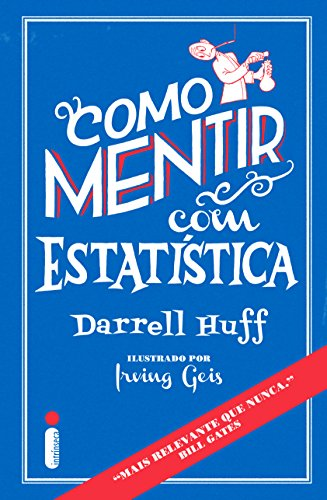
\includegraphics[width=0.3\textwidth]{imagens/livro.jpeg}
	\caption{Como Mentir com Estatística (Darrell Huff)}
\end{figure}

Então, não devemos encarar a Estatística como algo indecifrável ou como uma parte chata da Matemática que somos obrigados a engolir, mas como uma ciência que pode nos levar a algo novo e por muitos desconhecido. Muitas vezes serei repetitivo (e espero ser perdoado por isso) mas existe uma necessidade nessa repetição que é a de fixar os termos mais importantes.

\begin{theo}[Sobre os Exemplos]{}
	Antes de terminar gostaria de dizer que nesta apostila foram tratados exemplos sobre uma fictícia \textbf{Empresa ZzZ}, e obviamente espero que não exista tal Empresa.
\end{theo}

\section{Termos da Estatística}
Devemos possuir um vocabulário comum no qual tratarei daqui por diante:
\begin{itemize}[nolistsep]
	\item \textbf{População (N)}, definida como o todo que estamos interessados em estudar.
	\item \textbf{Amostra (n)}, uma porção da população para estudo.
	\item \textbf{Observação} um indivíduo completo da amostra (corresponde a uma linha em uma tabela ou planilha).
	\item \textbf{Variável de interesse ($V_{i}$)} característica obtida em cada observação (corresponde a uma coluna em uma tabela ou planilha) que temos o desejo de estudar.
	\item \textbf{Parâmetro} característica que descreve a população. Normalmente definido por letras gregas.
\end{itemize}

É importante observar que: \vspace{-1em}
\begin{itemize}
	\item \textbf{População}: conjunto constituído por todos os indivíduos que representam pelo menos uma característica comum, cujo comportamento nos interessa em analisar. \underline{Por exemplo}: O Diretor da Empresa ZzZ quer saber se os funcionários estão satisfeitos com os benefícios oferecidos. A população são todos os funcionários da Empresa ZzZ. Sendo assim o conceito de população depende do objetivo de estudo.
	\item \textbf{Amostra}: um subconjunto da população na qual podemos fazer usá-la para realizar inferências. \underline{Por exemplo}: O Diretor da Empresa ZzZ tem interesse em saber se todos os seus clientes gostam ou não do atendimento da Empresa. Não é possível perguntar a TODOS clientes dessa Empresa se eles gostam ou não. Então buscamos uma parte representativa dessa população, isto significa, perguntar somente a parte desses clientes.
	\item \textbf{Variável de Interesse}: característica a ser observada em cada indivíduo. Componentes sobre o qual serão observadas ou medidas as características. \underline{Por exemplo}: É necessário conhecer a média do índice de massa corporal (IMC) dos funcionários da Empresa ZzZ, sabendo que já existem registros cadastrados da altura e do peso de cada funcionário e que o IMC pode ser calculado por uma razão entre peso e o quadrado da altura do indivíduo. Nesse caso: \textbf{peso} e \textbf{altura} são nossas variáveis de interesse (outras características, como por exemplo: nome, idade ou gênero não nos interessa).
\end{itemize}

A estatística em si pode ser subdividida em: \vspace{-1em}
\begin{itemize}
	\item \textbf{Descritiva} - se ocupa em organizar, resumir e descrever ou apresentar as observações, que podem ser expressos em tabelas e gráficos.
	\item \textbf{Inferencial} - se ocupa em tirar conclusões sobre uma população a partir de uma amostra. A ferramenta básica nesse estudo é a \textbf{Probabilidade}.
\end{itemize}

\textbf{ESTATÍSTICA DESCRITIVA} se preocupa com a organização, apresentação e sintetização das observações. Utilizam gráficos, tabelas e medidas descritivas como ferramentas. Utilizada na etapa inicial da análise, destinada a obter informações que indicam possíveis modelos a serem utilizados numa fase final. As ferramentas utilizadas para isso são as bem conhecidas como tabelas de frequência, gráficos e o cálculo de medidas.

\textbf{ESTATÍSTICA INFERENCIAL} postula um conjunto de técnicas que permitem utilizar observações oriundas de uma amostra para generalizações sobre a população. Constitui esse conjunto de técnicas: determinação do número de observações (tamanho da amostra), esquema de seleção, confiança, significância e precisão das estimativas. A generalização é feita a partir do processo de estimação, porém não sem antes se antecipar um grau de certeza que a amostra tenha indivíduos que seriam de se esperar caso toda a população fosse estudada. Nesse sentido, uma ferramenta muito utilizada é a \textbf{probabilidade} no qual teremos condições de mensurar a fidedignidade de cada inferência feita com base na amostra.

\textbf{Fases do Método Estatístico:}
\begin{enumerate}[nolistsep]
	\item Definição do problema (se usaremos a População ou uma Amostra).
	\item Planejamento da pesquisa (definição das $V_{i}$).
	\item Coleta das observações.
	\item Resposta aos questionamentos realizados.
	\item Apresentação dos resultados.
\end{enumerate}

\subsection{Amostras}
Muitas vezes é impossível obter as observações de toda uma população, é neste momento que entra a amostra. Essa deve ser representativa, sua coleta bem como seu manuseio requer cuidados especiais para que os resultados não sejam distorcidos. Podemos obtê-las de várias formas, as mais comuns são:

\textbf{Amostragem Não-Probabilística}: Existe uma escolha deliberada dos indivíduos da amostra. Depende dos critérios do pesquisador. \vspace{-1em}
\begin{itemize}
	\item \textbf{Por Julgamento ou Intencional}: Requer um conhecimento da população e do subgrupo selecionado. Aplicação de questionários com os líderes dos funcionários da Empresa ZzZ.
	\item \textbf{Por Acessibilidade ou Conveniência}: Seleção dos indivíduos aos quais se tem acesso. Entrevistar os gerentes gerais da Empresa ZzZ a pedido do Diretor da Empresa.
	\item \textbf{Por Cotas}: classificar a população, determinar sua proporção por classe e fixar cotas em observância à proporção das classes consideradas (é a de maior rigor entre as amostragens não-probabilísticas), em geral é utilizada em pesquisa eleitoral e pesquisa de mercado. Um entrevistador quer entender como se comportam os clientes de um determinado produto da Empresa ZzZ e a população alvo é entre clientes entre 25 a 40 anos, o entrevistador pode dividir ainda mais os estratos de acordo com o gênero e selecionar somente 100 mulheres e homens pertencentes a esse grupo populacional.
\end{itemize}

\begin{table}[H]
	\centering 
	\begin{tabular}{m{3cm}|m{4cm}|m{5.5cm}}
		\textbf{Amostragem} & \textbf{Observações} & \textbf{Exemplo} \\
		\hline
		Por Julgamento ou Intencional & Através da escolha de um especialista & Para uma pesquisa considerar somente os funcionários que possuam mais de 10 anos na Empresa ZzZ. \\
		Por acessibilidade ou Conveniência & Por facilidade ou disposição. & No encontro anual dos funcionários da Empresa ZzZ foi anunciado que as 100 pessoas que se voluntariarem para um teste ganharão brindes. \\
		Por Cotas & Divisão da população em subgrupos, onde existem indivíduos de cada um & 58\% dos clientes interessados em comprar um produto da Empresa ZzZ tem entre 25 a 35 anos, os subgrupos devem ter as mesmas porcentagem de pessoas que pertencem esse respectivo grupo etário.
	\end{tabular}
\end{table}

\textbf{Amostragem Probabilística}: São amostragens em que a seleção é realizada de forma aleatória, de tal forma que cada indivíduo da população possui uma probabilidade real de fazer parte da amostra. São considerados métodos rigorosamente científicos.
\begin{itemize}
	\item \textbf{Aleatória Simples (AAS)}: se fundamenta no princípio de que todos os membros de uma população têm a mesma probabilidade de serem incluídos na amostra, indicado para populações homogêneas (pode ou não ocorrer reposição). Aplicar um questionário de satisfação sobre o ambiente de trabalho da Empresa ZzZ em 100 funcionários.
	\item \textbf{Sistemática}: A população deve ser ordenada de forma que sejam identificados. Para o mesmo exemplo anterior: Para encontrarmos os pontos onde faremos as coletas sistemáticas das amostras, seguir os seguintes passos:
	\begin{enumerate}
		\item calcular a razão $R = \nicefrac{N}{n}$ no qual \textbf{N} é o tamanho da população e \textbf{n} da amostra.
		\item Sortear um número qualquer ($N_{S}$) entre 1 a R.
		\item Obter os termos da seguinte forma: $N_{S}$, $N_{S} \times 2$, ..., $N_{S} \times n$
	\end{enumerate}
	Na prática: $N = 500$, $n = 100$, $R = 500/100 = 5$ e por exemplo $N_{S} = 3$. A amostra será: o 3º indivíduo, o 6º, o 9º e assim sucessivamente.
	\item \textbf{Estratificada}: Consiste em dividir a população em subgrupos mais homogêneos (estratos), de tal forma que haja uma homogeneidade dentro dos estratos e uma heterogeneidade entre eles. A definição dos estratos pode ser de acordo com sexo, idade, renda ou grau de instrução. Aplicar um questionário de satisfação sobre os serviços prestados pela Empresa ZzZ em 100 clientes que estão registrados em um banco de dados de 500 pessoas. Verifica-se que nessas 500 pessoas: 30\% são mulheres e 70\% são homens. Delimita-se que dos 500 clientes a serem entrevistados 150 sejam mulheres e 350 homens. Dizemos, neste caso, "gênero" é a variável de estratificação, ou que a população foi estratificada por "gênero". Pode assumir os seguintes tipos:
	\begin{enumerate}
		\item Uniforme - sorteio de um igual número de indivíduos.
		\item Proporcional - o número sorteado em cada estrato é proporcional a quantidade existente em cada estrato.
		\item Ótima - além de proporcional existe também a variação da $V_{i}$ no estrato que é medida pelo seu desvio padrão.
	\end{enumerate}
	\item \textbf{Por Conglomerados}: É um método muito utilizado por motivos de ordem prática econômica, onde divide-se uma população em pequenos grupos (conglomerados) e sorteia um número suficiente desses, cujos indivíduos constituirão a amostra. Este esquema é utilizado quando há uma subdivisão da população em grupos que sejam bastante semelhantes entre si, mas com fortes discrepâncias dentro dos grupos, de modo que cada um possa ser uma pequena representação da população de interesse específico. A amostragem é realizada em cima dos conglomerados, e não mais sobre os indivíduos da população. Diferente da Estratificada, este tipo é indicado em populações que apresentam muitos subgrupos e fica difícil extrair uma amostra de cada subgrupo.
\end{itemize}

\begin{table}[H]
	\centering 
	\begin{tabular}{m{3cm}|m{4cm}|m{5.5cm}}
		\textbf{Amostragem} & \textbf{Observações} & \textbf{Exemplo} \\
		\hline
		Aleatória Simples & Mesma probabilidade de seleção. & Selecionar 50 funcionários de uma fábrica da Empresa ZzZ por sorteio e verificar sua produtividade. \\
		Sistemática & Ocorre seguindo um intervalo fixo. & Em uma fila de itens produzidos nas fábricas da Empresa ZzZ, seleciona-se um item para revisão a cada 50 produzidos. \\
		Estratificada & Escolhas dentro de grupos distintos homogêneos. & Dentre 1000 funcionários da Empresa ZzZ, 200 são mulheres. Selecionar 50 funcionários para uma entrevista sendo que 10 deles devem ser mulheres. \\
		Por Conglomerados & Escolhas de grupos completos. & A Empresa ZzZ possui 50 setores distintos. Escolher 10 deles para realizar uma pesquisa de satisfação.
	\end{tabular}
\end{table}

Fatores que determinam qual será o tamanho da amostra:
\begin{itemize}
	\item \textbf{Nível de confiança}: quanto maior o nível, maior deve ser o tamanho da amostra.
	\item \textbf{Erro máximo permitido}: quanto menor o erro, maior deve ser o tamanho da amostra.
	\item \textbf{Variabilidade do fenômeno que está sendo investigado}: quanto maior a variabilidade, maior deve ser o tamanho da amostra.
\end{itemize}

\subsection{Variáveis de Interesse ($V_{i}$)}

\begin{figure}[H]
	\centering
	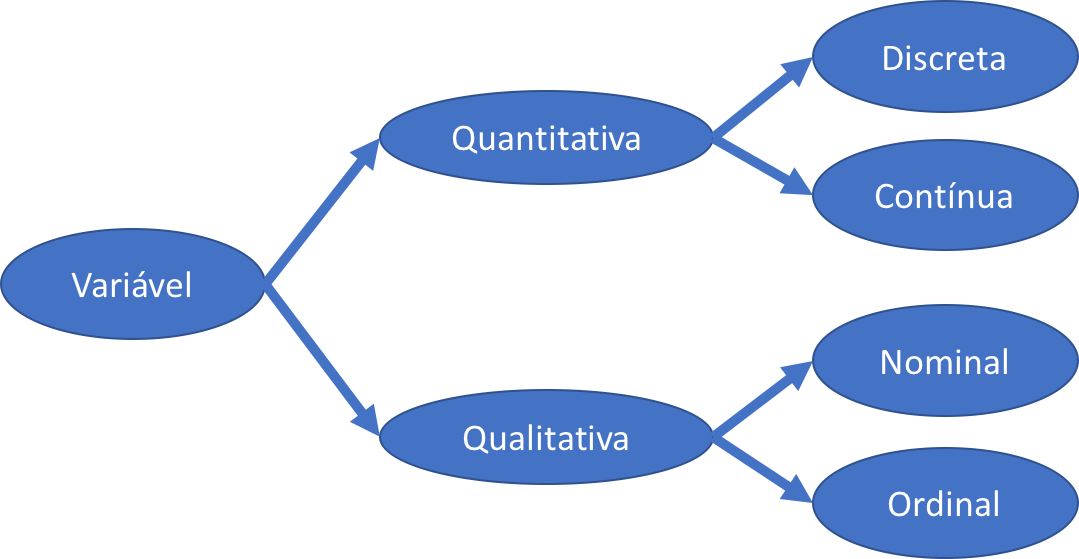
\includegraphics[width=0.6\textwidth]{imagens/tiposVariaveis.png}
	\caption{Tipos das Variáveis de Interesse}
\end{figure}

\textbf{Variável Quantitativa} são aquelas expressas por níveis, assumem valores em uma escala métrica definida por uma origem ou unidade. \vspace{-1em} 
\begin{itemize}
	\item \textbf{Discreta} assumem valores inteiros, um número finito de observações e expressa o valor de uma contagem, por exemplo: número de acidentes na Empresa ZzZ registrados no ano, total de peças defeituosas em lotes de produtos, quantidade de vendas realizadas em um período.
	\item \textbf{Contínua} podem assumir quaisquer valores reais em certo intervalo produzindo uma infinidade de valores, por exemplo: peso de um produto, viscosidade de um óleo, pressão dos pneus, peso e altura dos funcionários.
\end{itemize}

\textbf{Variável Qualitativa}, também chamadas de "Categóricas", são aquelas que assumem valores em categorias, classes ou rótulos. Sendo por natureza, não numéricas. Denotam características individuais das unidades sob análise e permitem estratificar essas para serem analisadas de acordo com outras variáveis. \vspace{-1em}
\begin{itemize}
	\item \textbf{Nominal} não apresentam sentido de ordem entre elas, por exemplo: tipo de máquina, naturalidade do funcionário, gênero, estado civil, raça.
	\item \textbf{Ordinal} apresentam uma ordem de relação pré-estabelecida, por exemplo: classe social, grau de desgaste, nível de escolaridade, grau de satisfação dos clientes.
\end{itemize}

\begin{theo}[A partir desse ponto]{}
	Não usaremos mais a palavra Variáveis de Interesse e somente seu acrônimo $V_{i}$, obviamente que também consideramos que em uma base de \underline{dados} (observe também que evitei utilizar essa palavra) só deve conter esse tipo de variável, pois elas é que são o nosso assunto a ser tratado.
\end{theo}

\section{Medidas}
Os valores $V_{i}$ podem ser medidos, dependendo de seu tipo. E com a realização dessas medições começamos a compreender o que representam as observações coletadas, nos orientarmos e obtermos as respostas aos mais variados questionamentos.

\subsection{Medidas de Tendência Central}
Permite conhecer o grau de concentração dos valores da $V_{i}$.

\textbf{Média}: pode ser de 3 tipos: \vspace{-1em}
\begin{itemize}
	\item Aritmética: $\bar{x} = \sum \nicefrac{x_{i}}{n}$
	\item Geométrica: $\bar{x} = \sqrt[n]{\prod_{i=1}^n{x_{i}}}$
	\item Harmônica: $\nicefrac{1}{\bar{x}} = \nicefrac{1}{n}\sum_{i=1}^n\nicefrac{1}{x_{i}}$
\end{itemize}

Relação entre as Médias: $MA \geq MG \geq MH$. Obviamente pela média aritmética ser a mais comum de todas, podemos nos referir a ela simplesmente por \textbf{média}. Porém é importante saber que existem outras, veja nesse exemplo que seus valores podem ser completamente diferentes.

\underline{Exemplo}: Calcular a MA, MG e MH para a seguinte $V_{i}$ com os valores ${1,2,5,3,4}$ \vspace{-1em}
\begin{itemize}
	\item MA: $\bar{x} = \sum \nicefrac{(1 + 2 + 5 + 3 + 4)}{5} = 3,0$
	\item MG: $\bar{x} = \sqrt[5]{(1 \times 2 \times 5 \times 3 \times 4)} \cong 2,605$
	\item MH: $\nicefrac{1}{\bar{x}} = \nicefrac{5}{\nicefrac{1}{1} + \nicefrac{1}{2} + \nicefrac{1}{5} + \nicefrac{1}{3} + \nicefrac{1}{4}} \cong 2,19$
\end{itemize}

\begin{theo}[Favor observar]{}
	Para as próximas medidas os valores da $V_{i}$ devem estar em ROL, ou seja ordenados.
\end{theo}

\textbf{Mediana}: Corresponde ao valor central, no qual contêm 50\% do total de observações.
\begin{itemize} \vspace{-1em}
	\item \textbf{n} ímpar: Calcular a posição central através de $PC = \nicefrac{n + 1}{2}$
	\item \textbf{n} par: Calcular as duas posições centrais através de $PC_{1} = \nicefrac{n + 1}{2}$ e $PC_{2} = \nicefrac{n + 1}{2} + 1$ e tirar a Média Aritmética.
\end{itemize}

Caso a $V_{i}$ estiver agrupada em classes, usamos a seguinte fórmula para calcular a mediana: \\[2mm]
$Md = l_{inf} + \nicefrac{ \nicefrac{n}{2} - f_{ac.Ant}}{f_{md} \times h}$

Sendo: \vspace{-1em}
\begin{itemize}[nolistsep]
	\item $l_{inf}$ limite inferior.
	\item $n$ somatório das frequências simples.
	\item $f_{ac.Ant}$ frequência acumulada até a da classe anterior a da mediana.
	\item $f_{md}$ frequência simples.
	\item $h$ amplitude do intervalo.
\end{itemize}

Podemos utilizar a seguinte Regra de 3 para chegar ao valor da mediana. A amplitude está para a frequência simples, assim como X está para a posição necessária para alcançar a mediana.

\textbf{Moda}: Corresponde ao valor que aparece com maior frequência na $V_{i}$, consequentemente o de maior probabilidade de ocorrência em um conjunto não agrupado em classes.

Tipos: \vspace{-1em}
\begin{itemize}[nolistsep]
	\item Amodal: não apresenta nenhum valor.
	\item Unimodal: um único valor.
	\item Bimodal: dois valores.
	\item Multimodal: apresenta mais de dois.
\end{itemize}

\subsection{Medidas Separatrizes}
Tem por objetivo dividir a quantidade de observações em n partes iguais, os mais utilizados são quartis ou percentis.

\textbf{Quartis}, dividem o conjunto em quatro partes iguais (de 25\% cada uma): \\
1º Quartil (1Q): parte as observações em 25\% para baixo e 75\% para cima. \\
2º Quartil (2Q): corresponde a mediana. \\
3º Quartil (3Q): parte as observações em 75\% para baixo e 25\% para cima.

\textbf{Percentis} (ou Centis), dividem o conjunto em cem partes iguais (de 1\% cada), e ao realizarmos as devidas associações temos que: \\
25º Percentil corresponde a 1Q. \\
50º Percentil corresponde a 2Q. \\
75º Percentil corresponde a 3Q.

Existem outras divisões que são chamadas de \textbf{Quintis} (em cinco partes iguais, sendo que cada grupo terá 20\%) e \textbf{Decis} (em dez partes iguais, sendo que cada grupo terá 10\%).

\subsection{Medidas de Dispersão}

\textbf{Intervalo} ou \textbf{Amplitude} (Range): a diferença entre o maior e menor número em uma observação. Por exemplo, considerando os valores: 10, 11, 13, 14 e 20. O valor 10 é o menor número e 20 o maior, temos que: $[10,20] = 10$

\textbf{Intervalo Inter-Quartil} (IQR): também chamado de \textit{mid-spread}, e divide ao meio o intervalo (50\%). Na prática é a diferença entre o 1º e o 3º Quartil.

\textbf{Semi Intervalo Inter-Quartil} (SIQR): é o valor da metade do IQR. Matematicamente falando é $(3Q - 1Q) \div 2$.

\textbf{Variância}: determina a variação em torno da média, esta medida pode ocorrer de 2 formas, pode ser a variação de uma população ou de uma amostra.

Fórmula para Variância de uma \textbf{População}: $\sigma^2 = \sum \nicefrac{(x_{i} - \mu)^2}{N}$

Fórmula para Variância de uma \textbf{Amostra}: $S^2 = \sum \nicefrac{(x_{i} - \bar{x})^2}{n - 1}$

\textbf{Desvio Padrão}: corresponde a dispersão de uma determinada série. Matematicamente é a raiz quadrada da variância.

Desvio padrão de uma \textbf{População}: $\sigma =\sqrt {\sum \nicefrac{(x_{i}-\mu)^2}{N}}$

Desvio padrão de uma \textbf{Amostra}: $S =\sqrt {\sum \nicefrac{(x_{i} - \bar{x})^2}{n - 1}}$

\textbf{Coeficiente de Variação} (CV): apresentada em percentual, representa a variação relativa da média. Utilizada para comparar dois ou mais observações de $V_{i}$ em diferentes unidades. Cuidado pois é extremamente sensível a presença de \textbf{outliers} (valores extremos). $CV = \nicefrac{\sigma}{\mu} \times 100$.

De forma geral se o resultado for:
\begin{itemize}[nolistsep]
	\item Menor ou igual a 15\% existe uma baixa dispersão: observações homogêneas.
	\item Entre 15 a 30\% uma média de dispersão.
	\item Maior que 30\% uma alta dispersão: observações heterogêneas.
\end{itemize}

\underline{Exemplo}: A Empresa ZzZ possui 2 seções: A com 20 empregados e B com 30, a média semanal de salário gasto é de R\$ 550,00 para A e R\$ 200,00 para B. O $\sigma$ de A é 7 enquanto que o $\sigma$ de B é 9.

Se usarmos somente a média salarial descobrimos que: \vspace{-1em}
\begin{itemize}
	\item Seção A: R\$ 11.000,00 ($20 \times 550$)
	\item Seção B: R\$ 6.000,00 ($30 \times 200$)
\end{itemize}

E ao analisarmos o CV: \vspace{-1em}
\begin{itemize}
	\item Seção A: $\nicefrac{7}{550} \times 100 = 1,27\%$
	\item Seção B: $\nicefrac{9}{200} \times 100 = 4,50\%$
\end{itemize}

Concluímos assim que a \textbf{Seção B} possui um custo menor (em média), porém que apesar existir uma baixa dispersão, esta seção possui uma maior diferença salarial entre seus funcionários.

\subsection{Prática Geral até aqui}
Vamos dar um tempo nas medições e descobrir algo de valor com o que aprendemos. A Empresa ZzZ deseja saber quais são os funcionários mais regulares em sua equipe na linha de montagem pois pretende promovê-los. Sendo assim, registramos a produção desses funcionários em uma semana de trabalho. Ao fim desse período, chegou-se à seguinte tabela:
\begin{figure}[H]
	\centering
	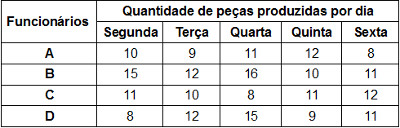
\includegraphics[width=0.6\textwidth]{imagens/tabelaFunc.jpg}
	\caption{Tabela de Produção de Cada Funcionário}
\end{figure}

Para conhecermos as primeiras observações sobre a produção de seus funcionários, fazemos o cálculo da média aritmética, mediana e moda e chegamos aos seguintes resultados:
\begin{table}[H]
	\centering 
	\begin{tabular}{c|l|l|l}
		\textbf{Funcionário} & \textbf{Média $\bar{x}$} & \textbf{Mediana $m_{d}$} & \textbf{Moda $m_{o}$} \\ \hline
		A & 10 & 10 & Amodal  \\ \hline
		B & 12,8 & 12 & Amodal \\ \hline
		C & 10,4 & 11 & 11 \\ \hline
		D & 11 & 11 & Amodal
	\end{tabular}
\end{table}

A partir desse cálculo, temos uma produção diária média de cada funcionário. Mas se observarmos bem a tabela, veremos que há valores distantes da média. O funcionário B, por exemplo, produz uma média de \textbf{12,8} peças por dia. No entanto, houve um dia em que produziu 16 peças e outro apenas 10 peças, já o Funcionário C é o único que é possível definir uma moda sendo os outros amodais. Será que este processo utilizado é suficiente para o propósito do dono da empresa? Então podemos considerar que somente o Funcionário C é regular?

Concluímos apenas que há variação entre a produção de cada funcionário. Mas e se tivéssemos mais de mil funcionários, ou se fosse observada a produção em um ano, será que conseguiríamos avaliar essa variação com tanta facilidade? A estatística nos apresenta outras medidas que permitem a análise de dispersão das observações. 

A variância nos mostra quão distantes os valores estão da média. Nesse caso, como estamos analisando todos os valores de cada funcionário, e não apenas uma "amostra", trata-se do cálculo da variância populacional ($\sigma^{2}$). Esse é obtido através da soma dos quadrados da diferença entre cada valor e a média da população($\mu$), dividida pela quantidade de indivíduos observados. Observamos o seguinte resultado:

$ \sigma^{2}(A) = 
\frac{(10 - 10)^{2} + (9 - 10)^{2} + (11 - 10)^{2} + (12 - 10)^{2} + (8 - 10)^{2}}{5}
= \frac{10}{5} \cong 2,0$

$\sigma^{2}(B) = \frac{(15 - 12,8)^{2} + (12 - 12,8)^{2} + (16 - 12,8)^{2} + (10 - 12,8)^{2} + (11 - 12,8)^{2}}{5} = \frac{26,8}{5} \cong 5,36$

$\sigma^{2}(C) = \frac{(11 - 10,4)^{2} + (10 - 10,4)^{2} + (8 - 10,4)^{2} + (11 - 10,4)^{2} + (12 - 10,4)^{2}}{5} = \frac{9,2}{5} \cong 1,84$

$\sigma^{2}(D) = \frac{(8 - 11)^{2} + (12 - 11)^{2} + (15 - 11)^{2} + (9 - 11)^{2} + (11 - 11)^{2}}{5} = \frac{30}{5} \cong 6,0$

\textbf{Observação}: Se fossemos trabalhar com variância amostral, deveríamos dividir pela quantidade de observações subtraída de um. Nesse exemplo teríamos: 5 - 1 = 4 dias.

Podemos notar que a produção dos funcionários C e A são mais uniforme e que de B e D mais desigual. Porém em algumas situações, apenas o cálculo da variância pode não ser suficiente, pois essa é uma medida de dispersão muito influenciada por valores que estão muito distantes da média. Além disso, o fato de a variância ser calculada "ao quadrado" causa certa camuflagem dos valores, dificultando a interpretação. Uma alternativa para solucionar esse problema é o Desvio Padrão.

O desvio padrão é o resultado positivo da raiz quadrada da variância. Na prática, indica qual o "erro" ao substituir um dos valores coletados pelo valor da média. Vamos agora calcular o desvio padrão ($\sigma$) da produção diária de cada funcionário:

$\sigma(A) = \sqrt{\sigma^{2}(A)} = \sqrt{2,0} \cong 1,41$

$\sigma(B) = \sqrt{\sigma^{2}(B)} = \sqrt{5,36} \cong 2,31$

$\sigma(C) = \sqrt{\sigma^{2}(C)} = \sqrt{1,84} \cong 1,35$

$\sigma(D) = \sqrt{\sigma^{2}(D)} = \sqrt{6,0} \cong 2,44$

Na utilização do desvio padrão na apresentação da média aritmética, temos a noção do quão "confiável" é esse valor. Uma outra forma de analisarmos os resultados seria através da amplitude das observações, no qual teríamos:

$ A[8,12] = 12 - 8 = 4$

$ B[10,16] = 16 - 10 = 6$

$ C[8,12] = 12 - 8 = 4$

$ D[8,15] = 15 - 8 = 7$

E observamos que realmente os funcionários A e C possuem uma menor diferença do que os funcionários B e D, sendo estes 2 primeiros mais constantes em sua produção. Devemos porém nos ater que a medida de Amplitude é um tanto limitada pois depende somente de valores externos. 

Por fim podemos concluir nosso relatório com o cálculo do Coeficiente de Variação que analisa a dispersão em termos relativos. Quanto menor for o valor do coeficiente de variação, mais homogêneas são as observações, ou seja, menor será a dispersão em torno da média. Então temos que:

$ CV(A) = \frac{1,41}{10} \times 100 = 14,14\%$

$ CV(B) = \frac{2,31}{12,8} \times 100 = 18,08\%$

$ CV(C) = \frac{1,35}{10,4} \times 100 = 13,04\%$

$ CV(D) = \frac{2,45}{11} \times 100 = 22,26\%$

O que mais uma vez confirma nossa previsão em dizer que os funcionários C e A são os mais regulares em sua produção.

\subsection{Medidas de Análise Bivariada}

\textbf{Covariância}: ou variância conjunta, é utilizada para medir qual o grau de interdependência que duas $V_{i}$ quaisquer (X e y) possuem.

$Cov(X,y) =  \nicefrac{\sum (X_{i} - \bar{X})(y_{i} - \bar{y})}{n(n -1)}$

Temos que: \vspace{-1em}
\begin{itemize}
	\item Uma covariância positiva significa que as variáveis se movem na mesma direção. Por exemplo: Taxa de alfabetização e Índice de Desenvolvimento Humano (IDH).
	\item Uma covariância positiva significa que as variáveis se movem em direções contrárias. Por exemplo: Índice de Pobreza e IDH.
	\item São independentes se esse número for zero (ou próximo). Por exemplo: Altura e IDH.
\end{itemize}

Quanto maior for esse número (positivamente ou negativamente) mais fortemente essas variáveis estão inter-relacionadas.

\underline{Exemplo}: A Empresa ZzZ possui 2 ações no mercado A e B que possuem o seguinte resultado: 
\begin{table}[H]
	\centering 
	\begin{tabular}{c|c|c}
		\textbf{Dia} & \textbf{Ação A} & \textbf{Ação B} \\ \hline
		1 & 20,00 & 30,00 \\ \hline
		2 & 27,00 & 42,00 \\ \hline
		3 & 21,00 & 49,00 \\ \hline
		4 & 14,00 & 41,00
	\end{tabular}
\end{table}

Desejamos saber como o preço da \textbf{Ação A} influencia na \textbf{Ação B}. Primeiro calculamos o preço de variação ($\nicefrac{diaAtual - diaAnt}{diaAnt}$), e temos o seguinte resultado:
\begin{table}[H]
	\centering 
	\begin{tabular}{c|c|c}
		\textbf{Dia} & \textbf{Ação A} & \textbf{Ação B} \\ \hline
		1 & - & - \\ \hline
		2 & 0,35 & 0,40 \\ \hline
		3 & -0,22 & 0,17 \\ \hline
		4 & -0,33 & -0,16
	\end{tabular}
\end{table}

Calculamos a média da Ação A: $\nicefrac{0,35 + (-0,22) + (-0,33)}{3} = -0,066$

Calculamos a média da Ação B: $\nicefrac{0,40 + 0,17 + (-0,16)}{3} = 0,136$

Aplicamos a primeira parte da Fórmula:
\begin{table}[H]
	\centering 
	\begin{tabular}{c|c|c}
		\textbf{$V_A - \bar{A}$} & \textbf{$V_B - \bar{B}$} & \textbf{$V_A - \bar{A} \times V_B - \bar{B}$} \\ \hline
		0,416 & 0,264 & 0,109824 \\ \hline
		-0,154 & 0,034 & -0,005236 \\ \hline
		-0,264 & -0,296 & 0,078144
	\end{tabular}
\end{table}

O somatório de valores multiplicados (última coluna) é: $0,182732$

E calculamos a covariância: $\nicefrac{0,182732}{3} = 0,06$

\subsubsection{Correlação de Pearson}
Mede a força de um relacionamento linear entre duas $V_{i}$ quantitativas. Seu valor está em um intervalo entre -1 e 1. Sendo também chamado de Correlação do Momento do Produto e dado pela fórmula:

$\rho = \nicefrac{Cov(X,y)}{\sigma(X) \times \sigma(y)}$

\underline{Exemplo}: Vamos retornar as ações da Empresa ZzZ e calculamos o Desvio Padrão de cada uma das ações:

Ação A: $\sigma(A) = \sqrt{\nicefrac{(0,35 - (-0,066))^2 + (0,22 - (-0,066))^2 + (-0,33 - (-0,066))^2}{3}} = 0,298$

Ação B: $\sigma(B) = \sqrt{\nicefrac{(0,4 - 0,136)^2 + (0,17 - 0,136)^2 + (-0,16 - 0,136)^2}{3}} = 0,230$

Então temos que: $\rho = \nicefrac{0,06}{(0,298 \times 0,230)} = 0,88$

Como o valor é próximo a +1 podemos concluir que existe uma positiva correlação entre os valores dessas ações.

\begin{theo}[Não confunda as palavras]{}
	\textbf{Correlação} e \textbf{Causalidade} não são sinônimos. Sendo que a primeira indica uma interdependência de duas ou mais variáveis. E a segunda uma ligação entre causa e efeito (algo acontece pois outra coisa causou).
\end{theo}

\subsubsection{Correlação de Spearman}
É uma classificação de correlação que utiliza medidas descritas pelo uso de uma função monótona\footnote{Em matemática, uma função entre dois conjuntos ordenados é monótona quando preserva (ou inverte) a relação de ordem.}. Seu valor também está em uma amplitude entre -1 e 1 e é utilizada com variáveis ordinais. Dado pela fórmula:

$r_S = 1 - \nicefrac{6 (\sum D^2)}{N (N^2-1)}$

\underline{Exemplo}: Aos funcionários da Empresa ZzZ foi aplicada duas provas: uma de Matemática e outra de Estatística para medir seu nível de conhecimento e obteve as seguintes notas:
\begin{table}[H]
	\centering 
	\begin{tabular}{c|c|c}
		\textbf{Funcionário} & \textbf{Matemática} & \textbf{Estatística} \\ \hline
		A & 75 & 82 \\ \hline
		B & 65 & 77 \\ \hline
		C & 83 & 93 \\ \hline
		D & 72 & 85 \\ \hline
		E & 88 & 89
	\end{tabular}
\end{table}

Passo 1, classificamos as notas:
\begin{table}[H]
	\centering 
	\begin{tabular}{c|c|c}
		\textbf{Funcionário} & \textbf{Matemática} & \textbf{Estatística} \\ \hline
		A & 3 & 4 \\ \hline
		B & 5 & 5 \\ \hline
		C & 2 & 1 \\ \hline
		D & 4 & 3 \\ \hline
		E & 1 & 2
	\end{tabular}
\end{table}

Passo 2, extraímos a diferença entre a classificação:
\begin{itemize}[nolistsep]
	\item Diferença de A: $D_A = 3 - 4 = -1$
	\item Diferença de B: $D_B = 5 - 5 = 0$
	\item Diferença de C: $D_C = 2 - 1 = 1$
	\item Diferença de D: $D_D = 4 - 3 = 1$
	\item Diferença de E: $D_E = 1 - 2 = -1$
\end{itemize}

Aplicamos a fórmula:

$r_S = 1 - \nicefrac{6 ((-1)^2 + 0^2 + 1^2 + (-1)^2)}{4 (4^2-1)} = 0,6$

E como é positivo e mais próximo a 1, podemos concluir que existe uma correlação é positiva entre as notas de Matemática e Estatística e produz uma função monótona crescente.

Resumidamente, a correlação é útil para descobrir o relacionamento entre $V_{i}$ e entender a força que age sobre elas. Coeficiente de correlação é o valor que nos diz sobre o tipo e a força de um relacionamento.
	
\section{Probabilidade}
Probabilidade é o estudo quantitativo da incerteza que nos ajuda a realizar uma ação otimizada de um determinado evento ocorrer ou não. A partir da seguinte afirmação: foi derrubado um aparelho no chão, vejamos os tipos de probabilidade: \vspace{-1em}
\begin{itemize}
	\item \textbf{a Priori}: antes de realizar qualquer tipo de teste, qual a probabilidade de um fato ter ocorrido ou não? Na afirmação: qual a chance deste aparelho ter quebrado? $P(A) = x\%$
	\item \textbf{Condicional}: qual a probabilidade de se saber um determinado fato após uma análise? Na afirmação: qual a chance de um técnico saber se o aparelho está ou não quebrado? $P(B \arrowvert A) = x\%$
	\item \textbf{Conjunta}: é a multiplicação das probabilidades acontecerem. Na afirmação: qual a chance do aparelho está quebrado e o técnico realmente saber que está quebrado? $P(A)P(B \arrowvert A) = x\%$  
	\item \textbf{a Posteriori}: probabilidade de um fato ter ocorrido ou não. Na afirmação: qual a chance do técnico saber de que o aparelho quebrou? $P(A) = x\%$
\end{itemize}

\subsection{Julgamento de Bernoulli}
Um experimento aleatório é chamado de \textbf{Julgamento de Bernoulli} se seguir as seguintes condições: \vspace{-1em}
\begin{itemize}
	\item Possui somente dois resultados possíveis: Sucesso ou Fracasso; Verdadeiro ou falso; Sim ou não.
	\item A probabilidade do resultado de qualquer estudo permanece fixa ao longo de todo o estudo.
	\item Os ensaios são estatisticamente independentes e aleatórios.
\end{itemize}

Um exemplo muito comum para um Julgamento de Bernoulli é o de lançar uma moeda. Existem apenas 2 resultados possíveis, isto é, cara ou coroa. Imaginemos que o evento de cara ser considerado sucesso (ou falha) e o evento de coroa sendo considerado um fracasso (ou sucesso). Uma moeda justa tem a probabilidade de sucesso 0,5 por definição, pois neste caso existem exatamente dois resultados possíveis.

Porém na prática descobrimos que abrangem quatro possibilidades na análise da qualidade do resultado (relativo ao que predizemos e o que realmente aconteceu). Por exemplo, foram feitas probabilidades a partir de registros médicos dos funcionários da Empresa ZzZ se o funcionário poderia (caso de sucesso ou doravante denominado Positivo) ou não desenvolver determinada doença (caso de falha ou doravante denominado Negativo). Ao analisar a qualidade da previsão dos resultados podemos considerar as seguintes condições: \vspace{-1em}
\begin{itemize}
	\item Verdadeiro Positivo ($P(+ \arrowvert D)$): resultado correto. O funcionário desenvolveu a doença e previmos que iria desenvolver.
	\item Falso Positivo ($P(- \arrowvert D)$): resultado incorreto. O funcionário desenvolveu a doença porém previmos que não iria desenvolver.
	\item Falso Negativo ($P(+ \arrowvert S)$): resultado incorreto. O funcionário não desenvolveu a doença (está saudável) porém previmos que iria desenvolver.
	\item Verdadeiro Negativo ($P(- \arrowvert S)$): resultado correto. O funcionário não desenvolveu a doença (está saudável) e previmos que não iria desenvolver.
\end{itemize}

Considerando os acertos da verificação temos que:

\textbf{Sensibilidade} - mede a capacidade do teste em identificar corretamente a doença entre aqueles que a possuem, ou seja, quão sensível é o teste. No exemplo, a sensibilidade é a fração dos que obtiveram resposta positiva no teste entre aqueles que possuem a doença, assim na fórmula aplicada aos doentes positivos:

$P(+ \arrowvert D) = \nicefrac{P( + \cap D)}{P(D)}$

\textbf{Especificidade} - mede a capacidade do teste em excluir corretamente aqueles que não possuem a doença, ou seja, quão específico é o teste. No exemplo, a especificidade é a fração dos que obtiveram resposta negativa no teste entre aqueles que não possuem a doença, assim na fórmula aplicada aos sadios negativos:

$P(- \arrowvert S) = \nicefrac{P( - \cap S)}{P(S)}$

\subsection{Axiomas da Probabilidade}
A probabilidade de qualquer experimento é sempre 0 a 1: \\
$0 \leq P(A) \leq 1$

A probabilidade de ocorrer o próprio evento sempre 1 ou 100\%: \\
$P(S) = 1$

Se A e B são eventos mutuamente exclusivos, então: \\
$P(A \cup B) = P(A) + P(B)$

\subsection{Teorema da Probabilidade Total}
A probabilidade condicional possui alguns teoremas, um deles é a \textbf{Probabilidade Total}, quando há várias condições que implicam nos resultados. Podemos utilizar este teorema para somar cada uma das condições. Para compreendê-lo, suponhamos que o espaço amostral S de um experimento em estudo esteja dividido em três eventos: $R_1$, $R_2$, $R_3$, conforme a figura:

\begin{figure}[H]
	\centering
	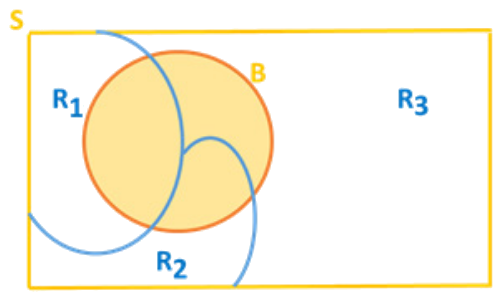
\includegraphics[width=0.5\textwidth]{imagens/espacoAmostral.png}
	\caption{Espaço Amostral S}
\end{figure}

Observamos que: $R_1 \cap R_2 = \emptyset$; $R_2 \cap R_3 = \emptyset$; $R_1 \cap R_3 = \emptyset$ e $R_1 \cup R_2 \cup R_3 = S$. Sendo B um evento qualquer dentro do espaço amostral S, existem três condições ($R_1$, $R_2$, $R_3$), para que ocorra e cada um deles com sua proporcionalidade dentro do espaço amostral. 

Podemos escrever: $B = B \cap S$. Como $S = R_1 \cup R_2 \cup R_3$, então esse evento B pode ser escrito como: 

$B = B \cap (R_1 \cup R_2 \cup R_3)$ 

ou ainda: 

$B = (B \cap R_1) \cup (B \cap R_2) \cup (B \cap R_3)$, 

ou em forma de probabilidade: 

$p(B) = p[(B \cap R_1) \cup (B \cap R_2) \cup (B \cap R_3)]$

Pelo fato de: $(B \cap R_1)$, $(B \cap R_2)$, $(B \cap R_3)$ serem eventos mutuamente exclusivos, podemos escrever: 

$p(B) = p(B \cap R_1) + p(B \cap R_2) + p(B \cap R_3)$

Pois as intersecções do 2º membro dessa expressão podem ser escritas pela fórmula da probabilidade condicional, ou seja:

$p(A \cap B) = p(\nicefrac{A}{B}) \times p(B)$

E substituindo, temos que: 

$p(B) = (p(\nicefrac{B}{R_1}) \times p(R_1)) + (p(\nicefrac{B}{R_2}) \times p(R_2)) + (p(\nicefrac{B}{R_3}) \times p(R_3))$

E este é o chamado de Teorema da Probabilidade Total, que ainda pode ser escrito de modo genérico (para “n” condições) por:

$(p(\nicefrac{B}{R_1}) \times p(R_1)) + (p(\nicefrac{B}{R_2}) \times p(R_2)) + ... + (p(\nicefrac{B}{R_n}) \times p(R_n))$

Por exemplo, as injetoras A e B são responsáveis por 70 e 30\%, respectivamente, da produção de plásticos de uma grande empresa de produtos domésticos. A máquina A produz 2\% de peças com defeito e a máquina B, por ser mais antiga, produz 8\% de peças defeituosas. Qual o percentual de peças defeituosas dessa empresa de produtos domésticos.

$p(d) = (p(\nicefrac{d}{A}) \times p(A)) + (p(\nicefrac{d}{B}) \times p(B)$) \\
$p(d) = (0,02 \times 0,7) + (0,08 \times 0,3) = 0,038$ ou 3,8\%

\subsection{Teorema de Bayes}
É a relação entre uma probabilidade condicional e a sua inversa. Representa uma das primeiras tentativas de modelar matematicamente a inferência estatística. Podemos defini-lo como um corolário do teorema da probabilidade total:

$p( \nicefrac{R_i}{B} ) = \nicefrac{[p( \nicefrac{B}{R_i} ) \times p(R_i)]}{[p( \nicefrac{B}{R_1} ) \times p(R_1) + p( \nicefrac{B}{R_2} ) \times p(R_2) + ... + p( \nicefrac{B}{R_n} ) \times p(R_n)]}$

O denominador da expressão é o \textbf{Teorema da Probabilidade Total}. Neste caso, a ocorrência de B por conta da condição $R_{i}$ está atrelada a sua probabilidade condicional, dividida pela total, e isso envolve quantas condições estiverem envolvidas.

\textbf{Por exemplo}: Na Empresa ZzZ as máquinas A e B são responsáveis por 60 e 40\% da produção, respectivamente. O departamento de qualidade afirma que os índices de peças defeituosas é de 4 e 6\%, respectivamente. Se uma peça defeituosa foi selecionada, qual a probabilidade dessa peça tenha sido produzida pela máquina B?

Sendo: \\
A = peça ter sido produzida na máquina A (responsável por 60\%) \\
B = peça ter sido produzida na máquina B (responsável por 40\%) \\
d = peça ser defeituosa

Temos que:

$p( \nicefrac{B}{d} ) = \nicefrac{[p( \nicefrac{d}{B} ) \times p(B)]}{[p( \nicefrac{d}{A} ) \times p(A) + p( \nicefrac{d}{B} ) \times p(B)]}$

$p( \nicefrac{B}{d} ) = \nicefrac{[0,06 \times 0,4]}{[(0,04 \times 0,6) + (0,06 \times 0,4)]} = 0,5$

Ou seja, temos 50\% de chance que a peça seja da máquina B.

\section{Distribuições e Probabilidade}
As distribuições de probabilidade discretas ou funções de massa de probabilidade ocorrem com o uso de variáveis aleatórias discretas. Essas funções atribuem uma probabilidade a cada ponto no espaço de amostra especificado. 

\subsection{Distribuição Geométrica}
Muitas ações que realizamos são repetitivas até atingir-se o sucesso. Digamos que tentaremos (no jogo de basquete) por várias vezes realizar uma cesta até conseguir acertar, ou ligaremos várias vezes para um local de alto congestionamento de ligações, até conseguir completar a ligação.

Situações como estas são representadas por uma distribuição denominada \textbf{Geométrica}, a qual é definida nas seguintes condições:
\begin{itemize}[nolistsep]
	\item Uma tentativa é repetida até que o sucesso ocorra.
	\item As tentativas são independentes uma das outras.
	\item A probabilidade de sucesso "p" é constante para cada tentativa.
\end{itemize}

A probabilidade de que o primeiro sucesso ocorra na tentativa número "x" é dada por:

$p(x) = p \times q^{x - 1}$, onde $q = 1 - p$.

\subsection{Comparativo da Distribuição de Poisson e Binomial}
Com base nos princípios da distribuição de Poisson, fica claro que essa está relacionada com a distribuição binomial, tanto que há alguns exemplos que podem ser calculados tanto pela binomial como Poisson que os resultados serão muito próximos. Por exemplo, suponha que uma máquina da Empresa ZzZ produz 9 peças com defeito a cada 1.000 peças produzidas, calcular a probabilidade de que, em 200 peças escolhidas aleatoriamente, sejam encontradas 8 com defeito:

Pela Distribuição Binomial:

$p(x) = \frac{n!}{(n - x)! x!} \times p^x \times q^{n - x}$

sendo: $p = \frac{9}{1000} = 0,009; q = 1 - p = 0,991$

$p(8) = \frac{200!}{(200 - 8)! 8!} \times 0,009^8 \times 0,991^192 = 0,00042$

Pela Distribuição de Poisson:

$p(x) = \frac{\mu^x \times e^{-\mu}}{x!}$

sendo: $\mu = n \times p = 200 \times 0,009 = 1,8; e = 2,71828$

$p(8) = \frac{1,8^8 \times 2,71828^{-1,8}}{8!} = 0,00045$

As duas formas de cálculos, os resultados apresentam praticamente os mesmos valores, uma vez que as condições para a aproximação $n > 30$ e a probabilidade $p < 0,05$ estão satisfeitas.

\subsection{Distribuição Normal}
\textbf{Frederick Gauss} (em meados do século XIX) com seus estudos sobre eventos da natureza, observou um comportamento padrão entre suas amostras. Posteriormente foi apresentado como a \textbf{Curva de Gauss} e mostrava que grande parte dos eventos ficam em torno de um valor médio (lembra de \textbf{Galton}), com uma certa variabilidade.

Uma distribuição estatística é uma função que define uma curva, e a área sob essa curva determina a probabilidade de ocorrer o evento por ela correlacionado. E o que é distribuição normal? Também conhecida como distribuição gaussiana, é uma curva simétrica em torno do seu ponto médio, apresentando assim um formato de sino. 
\begin{figure}[H]
	\centering
	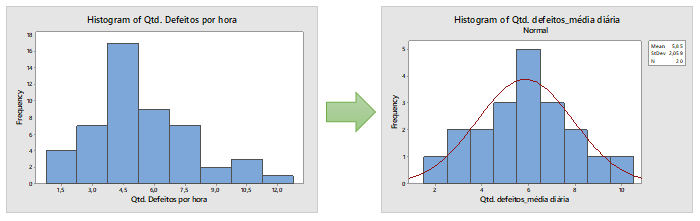
\includegraphics[width=0.85\textwidth]{imagens/curvaGaussiana.png}
	\caption{Curva Gaussiana}
\end{figure}

A curva de distribuição normal representa o comportamento de diversos processos nas empresas e muitos fenômenos comuns, como por exemplo, altura ou peso de uma população, a pressão sanguínea de um grupo de pessoas, o tempo que um grupo de estudantes gasta para realizar uma prova. A distribuição normal pode ser usada para aproximar distribuições discretas de probabilidade, como por exemplo a distribuição binomial. Além disso, serve também como base para a inferência estatística clássica. Nela, a média, mediana e moda possuem o mesmo valor.

Uma Distribuição Normal apresenta as seguintes características:
\begin{figure}[H]
	\centering
	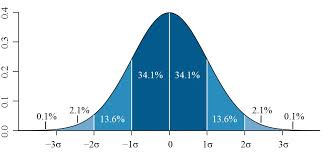
\includegraphics[width=0.70\textwidth]{imagens/sigmaDistNormal.jpeg}
	\caption{Distribuição das Observações}
\end{figure}

Sendo que o valor de $\mu$ é o ponto central e representado pelo valor $0$, além disso na Distribuição Normal o $\sigma$ é sempre igual a $1$, então a esquerda temos os valores $[-1, -2, -3]$ e a direita os valores $[1, 2, 3]$. Deste modo com as tabelas descritas ao final dessa seção é possível calcularmos qualquer área dessa curva.

\subsubsection{Tabelas Z}
Já sabemos que quase nenhum conjunto de observações segue um padrão perfeito da Distribuição Normal de valores, isso é: $[-3, -2, -1, 0, 1, 2, 3]$. Devemos converter para esse modo, e para isso usamos as tabelas Z, esse processo é chamado de \textbf{Normalização}. 

\underline{Por exemplo}: A Empresa ZzZ realizou uma prova entre seus funcionários e o resultado foram notas normalmente distribuídas. Dados que $\mu = 75$ e $\sigma = 10$. Qual a probabilidade de um determinado funcionário ter obtido uma nota acima de 60?

1º Passo - Converter para uma Distribuição Normal

$z = \frac{X - \mu}{\sigma} = \frac{60 - 75}{10} = \frac{-15}{10} = -1,5$

2º Passo - Achar na tabela (veja ao final dessa apostila) o ponto correspondente ao localizado: -1,5 na linha e 0 na coluna e temos o valor: $0,0668$ ou seja temos que a área a esquerda corresponde a $6,68\%$ da curva total. 

Porém observamos que o problema deseja saber os resultados acima desse valor, sendo assim $93,32\%$ dos funcionários podem ter obtido uma nota acima de 60 na prova.

\section{Conclusão}
No mundo da incerteza, a saída de qualquer evento é desconhecida com antecedência e isso dificulta o processo na tomada das decisões. É importante entender a estrutura dessa incerteza para termos uma ideia sobre o risco e a recompensa associados em cada ação executada. 

Ao considerar que o gerente da Empresa ZzZ quer estimar o número médio de peças produzidos pela fábrica em uma hora. A estatística ou métrica usada para medir o valor do parâmetro populacional (ou seja, média, mediana, variância ou outras) é chamado de \textbf{Estimador}.

Um \textbf{evento} é o resultado de um experimento. Um \textbf{experimento} é um processo que é realizado para entender e observar possíveis resultados. E o conjunto de todos os resultados de um experimento é chamado de \textbf{espaço amostral}. Existe toda uma nova linguagem para aprender e não desejo em criar um pensamento errado que esta apostila abrange toda a estatística. Permita-se explorar esse novo mundo e que essa seja apenas o começo da estrada que devemos percorrer a partir de agora. 

Sou um entusiasta do mundo \textbf{Open Source} e novas tecnologias. Qual a diferença entre Livre e Open Source? \underline{Livre} significa que esta apostila é gratuita e pode ser compartilhada a vontade. \underline{Open Source} além de livre todos os arquivos que permitem a geração desta (chamados de arquivos fontes) devem ser disponibilizados para que qualquer pessoa possa modificar ao seu prazer, gerar novas, complementar ou fazer o que quiser. Os fontes da apostila (que foi produzida com o LaTex) está disponibilizado no GitHub \cite{github}, assim baixar, alterar e usar. Veja ainda outros artigos que publico sobre tecnologia através do meu Blog Oficial \cite{fernandoanselmo}.

%-----------------------------------------------------------------------------
% REFERÊNCIAS
%-----------------------------------------------------------------------------

\begin{thebibliography}{3}
	\bibitem{fernandoanselmo} 
	Fernando Anselmo - Blog Oficial de Tecnologia \\
	\url{http://www.fernandoanselmo.blogspot.com.br/}
	
	\bibitem{publicacao} 
	Encontre essa e outras publicações em \\
	\url{https://cetrex.academia.edu/FernandoAnselmo}

	\bibitem{github} 
	Repositório para os fontes da apostila \\
	\url{https://github.com/fernandoans/publicacoes}	
\end{thebibliography}

\newpage
\begin{figure}[!htb]
	\centering
	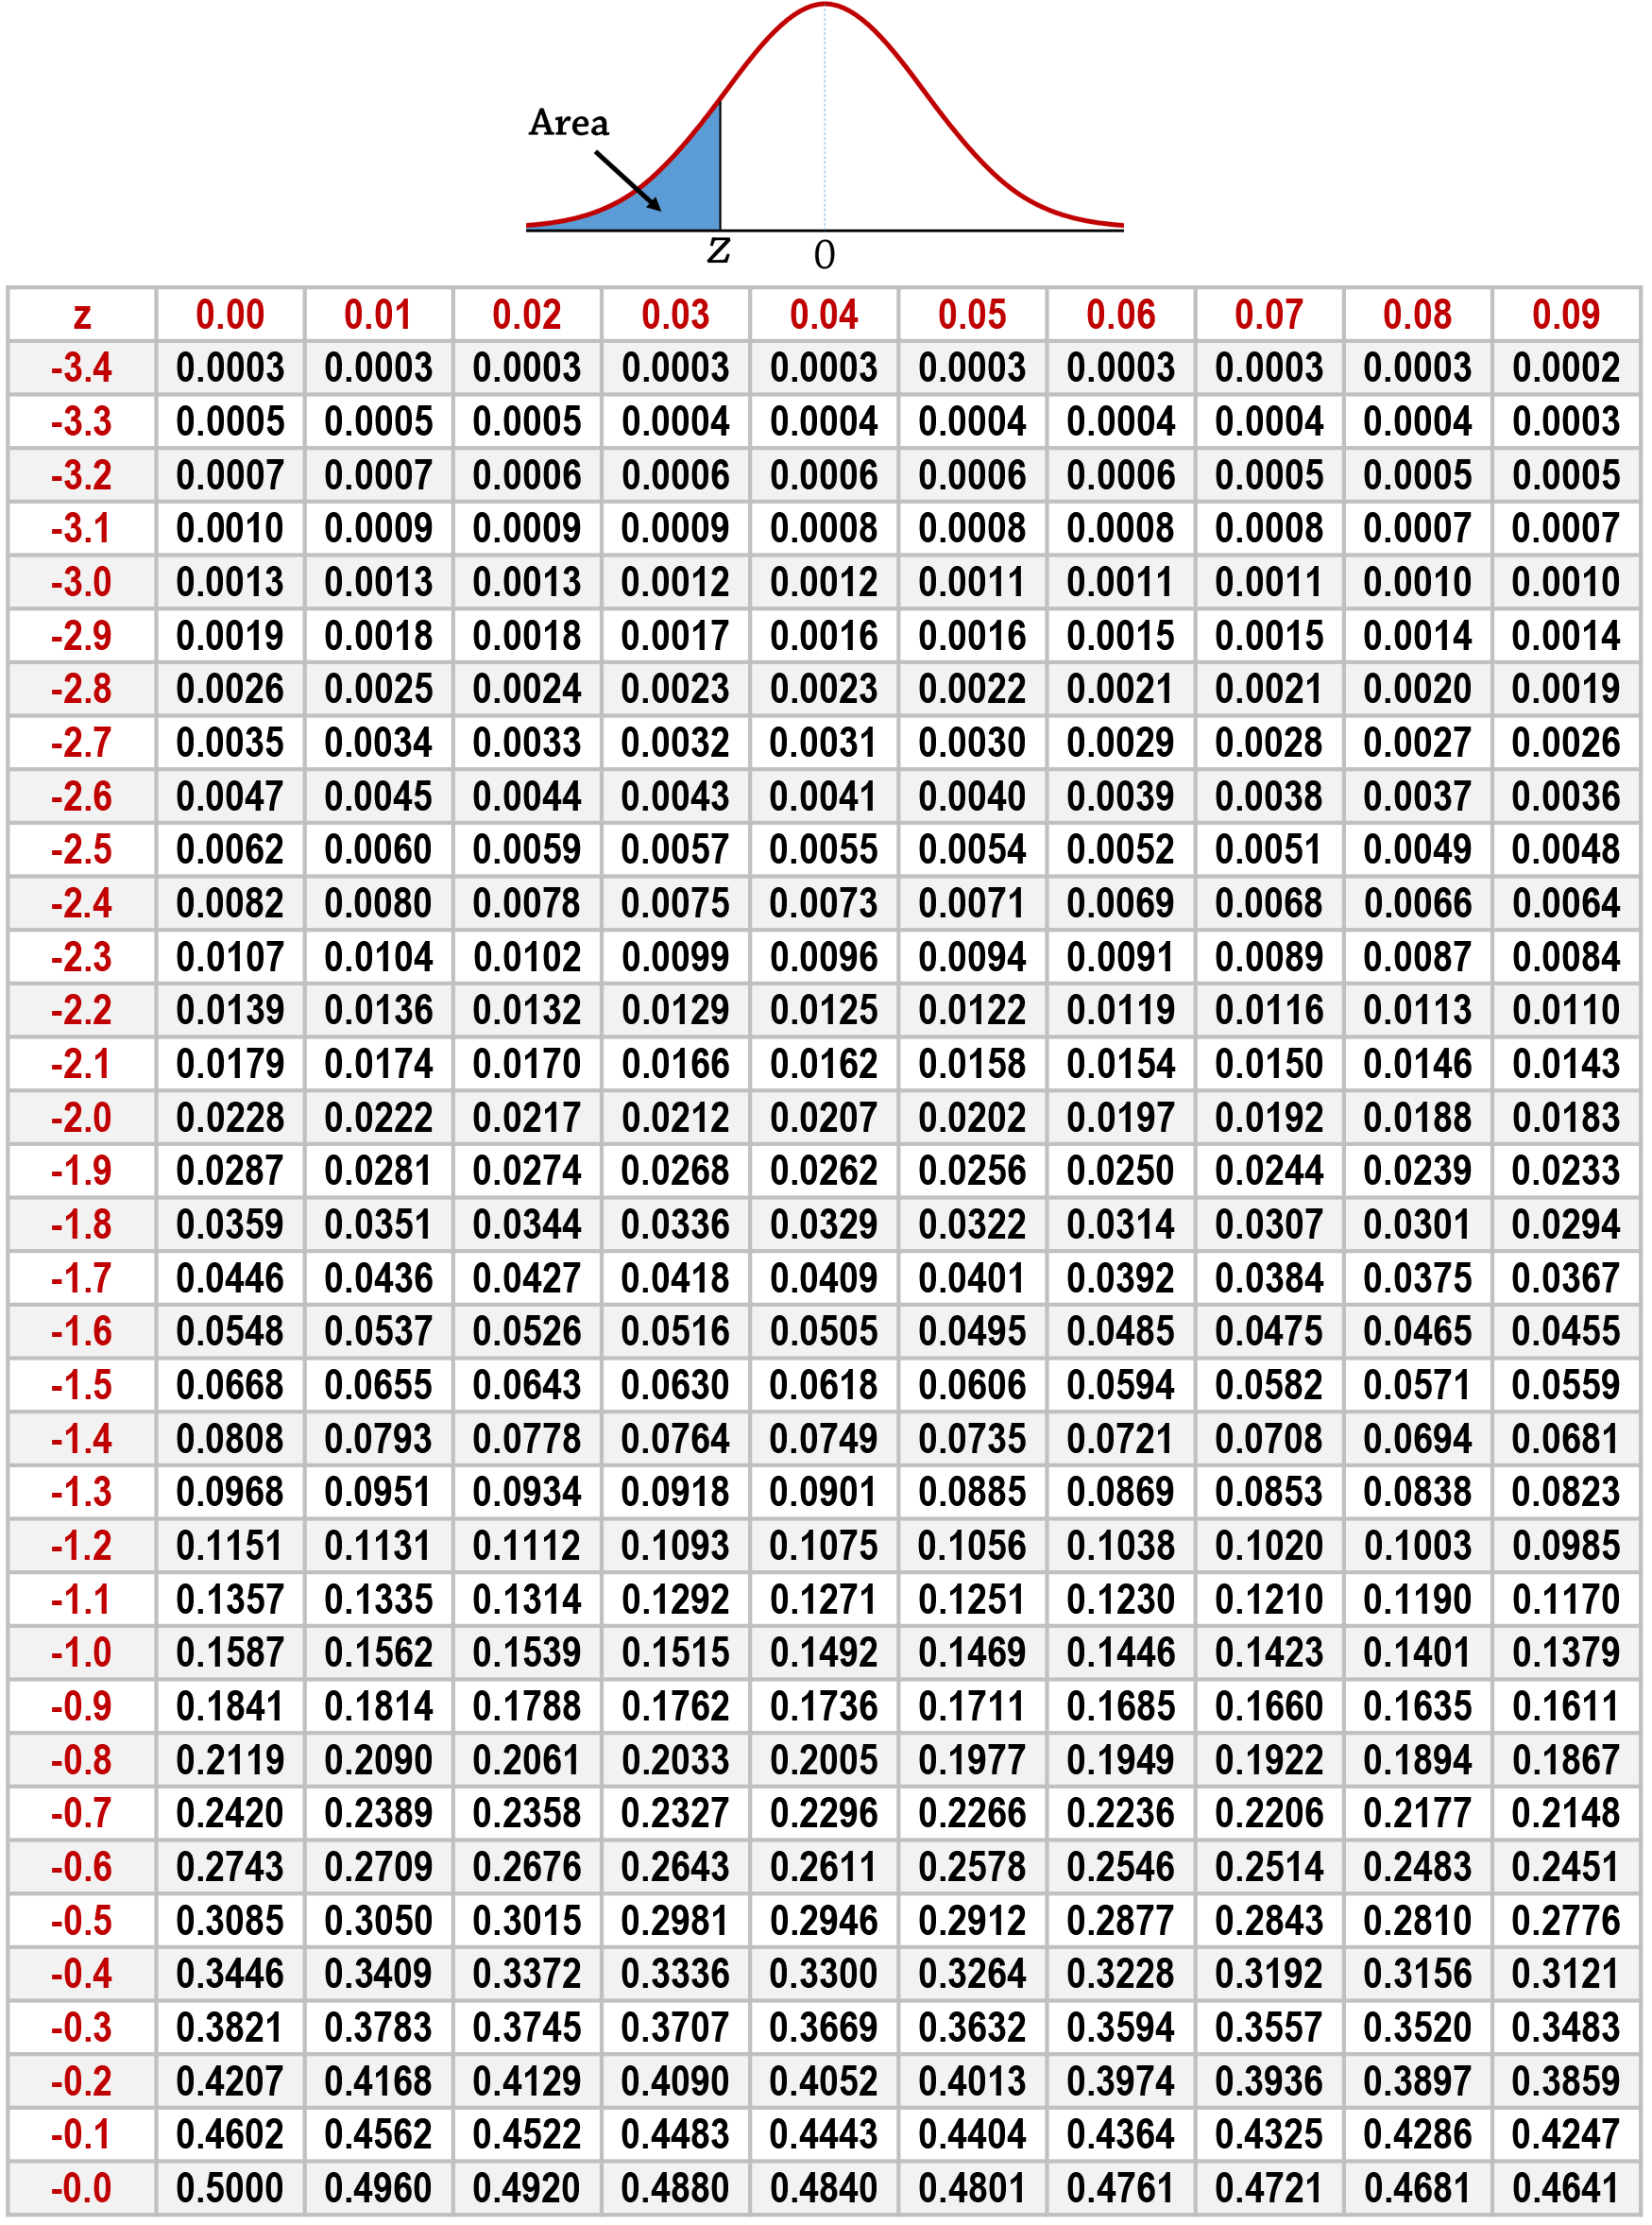
\includegraphics[width=1.0\textwidth]{imagens/ztable.png}
	\caption{Tabela Z para o ponto a esquerda de $\sigma$}
\end{figure}

\newpage
\begin{figure}[!htb]
	\centering
	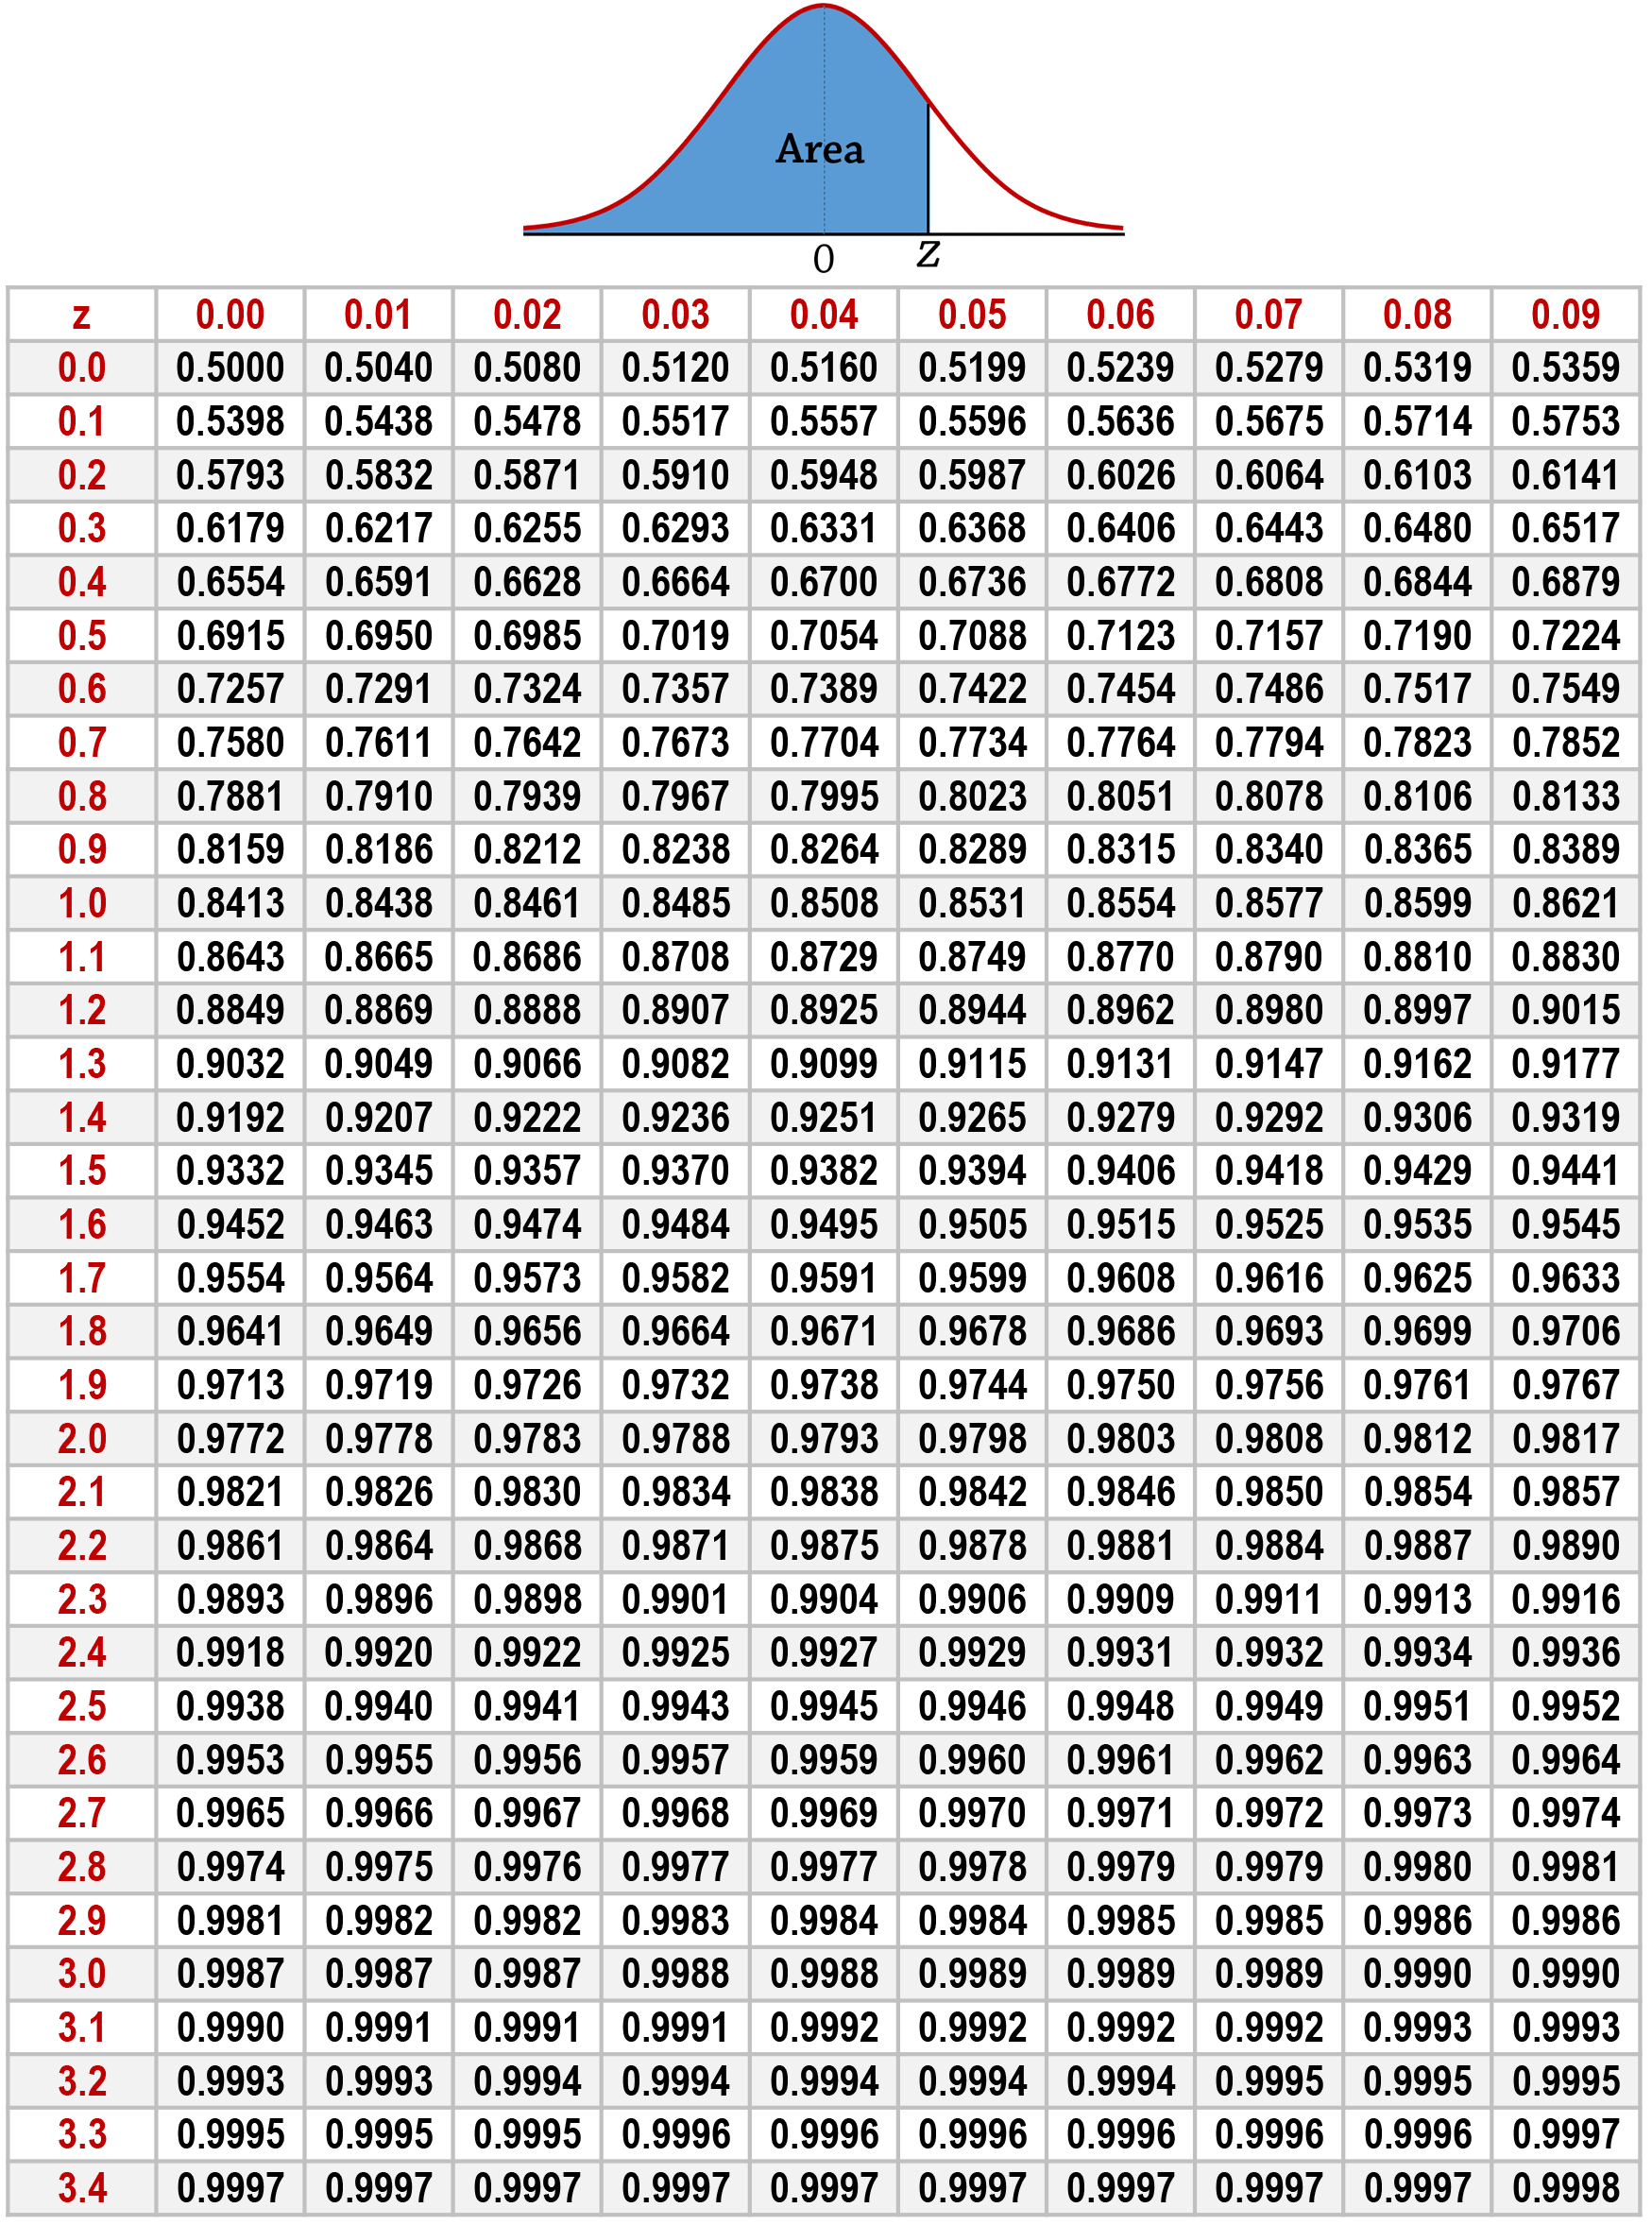
\includegraphics[width=1.0\textwidth]{imagens/ztable2.png}
	\caption{Tabela Z para o ponto a direita de $\sigma$}
\end{figure}

\end{document}
	